% Options for packages loaded elsewhere
\PassOptionsToPackage{unicode}{hyperref}
\PassOptionsToPackage{hyphens}{url}
\PassOptionsToPackage{dvipsnames,svgnames,x11names}{xcolor}
%
\documentclass[
  letterpaper,
  DIV=11,
  numbers=noendperiod]{scrartcl}

\usepackage{amsmath,amssymb}
\usepackage{lmodern}
\usepackage{iftex}
\ifPDFTeX
  \usepackage[T1]{fontenc}
  \usepackage[utf8]{inputenc}
  \usepackage{textcomp} % provide euro and other symbols
\else % if luatex or xetex
  \usepackage{unicode-math}
  \defaultfontfeatures{Scale=MatchLowercase}
  \defaultfontfeatures[\rmfamily]{Ligatures=TeX,Scale=1}
\fi
% Use upquote if available, for straight quotes in verbatim environments
\IfFileExists{upquote.sty}{\usepackage{upquote}}{}
\IfFileExists{microtype.sty}{% use microtype if available
  \usepackage[]{microtype}
  \UseMicrotypeSet[protrusion]{basicmath} % disable protrusion for tt fonts
}{}
\makeatletter
\@ifundefined{KOMAClassName}{% if non-KOMA class
  \IfFileExists{parskip.sty}{%
    \usepackage{parskip}
  }{% else
    \setlength{\parindent}{0pt}
    \setlength{\parskip}{6pt plus 2pt minus 1pt}}
}{% if KOMA class
  \KOMAoptions{parskip=half}}
\makeatother
\usepackage{xcolor}
\usepackage[normalem]{ulem}
\setlength{\emergencystretch}{3em} % prevent overfull lines
\setcounter{secnumdepth}{-\maxdimen} % remove section numbering
% Make \paragraph and \subparagraph free-standing
\ifx\paragraph\undefined\else
  \let\oldparagraph\paragraph
  \renewcommand{\paragraph}[1]{\oldparagraph{#1}\mbox{}}
\fi
\ifx\subparagraph\undefined\else
  \let\oldsubparagraph\subparagraph
  \renewcommand{\subparagraph}[1]{\oldsubparagraph{#1}\mbox{}}
\fi

\usepackage{color}
\usepackage{fancyvrb}
\newcommand{\VerbBar}{|}
\newcommand{\VERB}{\Verb[commandchars=\\\{\}]}
\DefineVerbatimEnvironment{Highlighting}{Verbatim}{commandchars=\\\{\}}
% Add ',fontsize=\small' for more characters per line
\usepackage{framed}
\definecolor{shadecolor}{RGB}{241,243,245}
\newenvironment{Shaded}{\begin{snugshade}}{\end{snugshade}}
\newcommand{\AlertTok}[1]{\textcolor[rgb]{0.68,0.00,0.00}{#1}}
\newcommand{\AnnotationTok}[1]{\textcolor[rgb]{0.37,0.37,0.37}{#1}}
\newcommand{\AttributeTok}[1]{\textcolor[rgb]{0.40,0.45,0.13}{#1}}
\newcommand{\BaseNTok}[1]{\textcolor[rgb]{0.68,0.00,0.00}{#1}}
\newcommand{\BuiltInTok}[1]{\textcolor[rgb]{0.00,0.23,0.31}{#1}}
\newcommand{\CharTok}[1]{\textcolor[rgb]{0.13,0.47,0.30}{#1}}
\newcommand{\CommentTok}[1]{\textcolor[rgb]{0.37,0.37,0.37}{#1}}
\newcommand{\CommentVarTok}[1]{\textcolor[rgb]{0.37,0.37,0.37}{\textit{#1}}}
\newcommand{\ConstantTok}[1]{\textcolor[rgb]{0.56,0.35,0.01}{#1}}
\newcommand{\ControlFlowTok}[1]{\textcolor[rgb]{0.00,0.23,0.31}{#1}}
\newcommand{\DataTypeTok}[1]{\textcolor[rgb]{0.68,0.00,0.00}{#1}}
\newcommand{\DecValTok}[1]{\textcolor[rgb]{0.68,0.00,0.00}{#1}}
\newcommand{\DocumentationTok}[1]{\textcolor[rgb]{0.37,0.37,0.37}{\textit{#1}}}
\newcommand{\ErrorTok}[1]{\textcolor[rgb]{0.68,0.00,0.00}{#1}}
\newcommand{\ExtensionTok}[1]{\textcolor[rgb]{0.00,0.23,0.31}{#1}}
\newcommand{\FloatTok}[1]{\textcolor[rgb]{0.68,0.00,0.00}{#1}}
\newcommand{\FunctionTok}[1]{\textcolor[rgb]{0.28,0.35,0.67}{#1}}
\newcommand{\ImportTok}[1]{\textcolor[rgb]{0.00,0.46,0.62}{#1}}
\newcommand{\InformationTok}[1]{\textcolor[rgb]{0.37,0.37,0.37}{#1}}
\newcommand{\KeywordTok}[1]{\textcolor[rgb]{0.00,0.23,0.31}{#1}}
\newcommand{\NormalTok}[1]{\textcolor[rgb]{0.00,0.23,0.31}{#1}}
\newcommand{\OperatorTok}[1]{\textcolor[rgb]{0.37,0.37,0.37}{#1}}
\newcommand{\OtherTok}[1]{\textcolor[rgb]{0.00,0.23,0.31}{#1}}
\newcommand{\PreprocessorTok}[1]{\textcolor[rgb]{0.68,0.00,0.00}{#1}}
\newcommand{\RegionMarkerTok}[1]{\textcolor[rgb]{0.00,0.23,0.31}{#1}}
\newcommand{\SpecialCharTok}[1]{\textcolor[rgb]{0.37,0.37,0.37}{#1}}
\newcommand{\SpecialStringTok}[1]{\textcolor[rgb]{0.13,0.47,0.30}{#1}}
\newcommand{\StringTok}[1]{\textcolor[rgb]{0.13,0.47,0.30}{#1}}
\newcommand{\VariableTok}[1]{\textcolor[rgb]{0.07,0.07,0.07}{#1}}
\newcommand{\VerbatimStringTok}[1]{\textcolor[rgb]{0.13,0.47,0.30}{#1}}
\newcommand{\WarningTok}[1]{\textcolor[rgb]{0.37,0.37,0.37}{\textit{#1}}}

\providecommand{\tightlist}{%
  \setlength{\itemsep}{0pt}\setlength{\parskip}{0pt}}\usepackage{longtable,booktabs,array}
\usepackage{calc} % for calculating minipage widths
% Correct order of tables after \paragraph or \subparagraph
\usepackage{etoolbox}
\makeatletter
\patchcmd\longtable{\par}{\if@noskipsec\mbox{}\fi\par}{}{}
\makeatother
% Allow footnotes in longtable head/foot
\IfFileExists{footnotehyper.sty}{\usepackage{footnotehyper}}{\usepackage{footnote}}
\makesavenoteenv{longtable}
\usepackage{graphicx}
\makeatletter
\def\maxwidth{\ifdim\Gin@nat@width>\linewidth\linewidth\else\Gin@nat@width\fi}
\def\maxheight{\ifdim\Gin@nat@height>\textheight\textheight\else\Gin@nat@height\fi}
\makeatother
% Scale images if necessary, so that they will not overflow the page
% margins by default, and it is still possible to overwrite the defaults
% using explicit options in \includegraphics[width, height, ...]{}
\setkeys{Gin}{width=\maxwidth,height=\maxheight,keepaspectratio}
% Set default figure placement to htbp
\makeatletter
\def\fps@figure{htbp}
\makeatother

\KOMAoption{captions}{tableheading}
\makeatletter
\makeatother
\makeatletter
\makeatother
\makeatletter
\@ifpackageloaded{caption}{}{\usepackage{caption}}
\AtBeginDocument{%
\ifdefined\contentsname
  \renewcommand*\contentsname{Содержание}
\else
  \newcommand\contentsname{Содержание}
\fi
\ifdefined\listfigurename
  \renewcommand*\listfigurename{Список Иллюстраций}
\else
  \newcommand\listfigurename{Список Иллюстраций}
\fi
\ifdefined\listtablename
  \renewcommand*\listtablename{Список Таблиц}
\else
  \newcommand\listtablename{Список Таблиц}
\fi
\ifdefined\figurename
  \renewcommand*\figurename{Рисунок}
\else
  \newcommand\figurename{Рисунок}
\fi
\ifdefined\tablename
  \renewcommand*\tablename{Таблица}
\else
  \newcommand\tablename{Таблица}
\fi
}
\@ifpackageloaded{float}{}{\usepackage{float}}
\floatstyle{ruled}
\@ifundefined{c@chapter}{\newfloat{codelisting}{h}{lop}}{\newfloat{codelisting}{h}{lop}[chapter]}
\floatname{codelisting}{Список}
\newcommand*\listoflistings{\listof{codelisting}{Список Каталогов}}
\makeatother
\makeatletter
\@ifpackageloaded{caption}{}{\usepackage{caption}}
\@ifpackageloaded{subcaption}{}{\usepackage{subcaption}}
\makeatother
\makeatletter
\@ifpackageloaded{tcolorbox}{}{\usepackage[many]{tcolorbox}}
\makeatother
\makeatletter
\@ifundefined{shadecolor}{\definecolor{shadecolor}{rgb}{.97, .97, .97}}
\makeatother
\makeatletter
\makeatother
\ifLuaTeX
\usepackage[bidi=basic]{babel}
\else
\usepackage[bidi=default]{babel}
\fi
\babelprovide[main,import]{russian}
% get rid of language-specific shorthands (see #6817):
\let\LanguageShortHands\languageshorthands
\def\languageshorthands#1{}
\ifLuaTeX
  \usepackage{selnolig}  % disable illegal ligatures
\fi
\IfFileExists{bookmark.sty}{\usepackage{bookmark}}{\usepackage{hyperref}}
\IfFileExists{xurl.sty}{\usepackage{xurl}}{} % add URL line breaks if available
\urlstyle{same} % disable monospaced font for URLs
\hypersetup{
  pdftitle={our autumn quarto smaller},
  pdflang={ru},
  colorlinks=true,
  linkcolor={blue},
  filecolor={Maroon},
  citecolor={Blue},
  urlcolor={Blue},
  pdfcreator={LaTeX via pandoc}}

\title{our autumn quarto smaller}
\author{}
\date{}

\begin{document}
\maketitle
\ifdefined\Shaded\renewenvironment{Shaded}{\begin{tcolorbox}[frame hidden, interior hidden, borderline west={3pt}{0pt}{shadecolor}, enhanced, boxrule=0pt, breakable, sharp corners]}{\end{tcolorbox}}\fi

\hypertarget{ux432ux44bux434ux435ux43bux435ux43dux438ux435-ux43fux43eux43bux443ux436ux438ux440ux43dux44bux43c-ux438-ux432ux44bux434ux435ux43bux435ux43dux438ux435-ux43aux443ux440ux441ux438ux432ux43eux43c}{%
\subsection{Выделение полужирным и выделение
курсивом}\label{ux432ux44bux434ux435ux43bux435ux43dux438ux435-ux43fux43eux43bux443ux436ux438ux440ux43dux44bux43c-ux438-ux432ux44bux434ux435ux43bux435ux43dux438ux435-ux43aux443ux440ux441ux438ux432ux43eux43c}}

\textbf{Полужирный} вот такой и \textbf{полужирный} вот такой

\emph{Курсив} вот такой и \emph{курсив} вот такой

\hypertarget{ux43fux43eux434ux437ux430ux433ux43eux43bux43eux432ux43eux43a}{%
\subsubsection{Подзаголовок}\label{ux43fux43eux434ux437ux430ux433ux43eux43bux43eux432ux43eux43a}}

\hypertarget{ux43fux43eux434ux437ux430ux433ux43eux43bux43eux432ux43eux43a-ux43fux43eux43cux435ux43dux44cux448ux435}{%
\paragraph{Подзаголовок
поменьше}\label{ux43fux43eux434ux437ux430ux433ux43eux43bux43eux432ux43eux43a-ux43fux43eux43cux435ux43dux44cux448ux435}}

\hypertarget{ux43fux43eux434ux437ux430ux433ux43eux43bux43eux432ux43eux43a-ux432ux43eux43eux431ux449ux435-ux43cux430ux43bux435ux43dux44cux43aux438ux439-ux436ux435ux441ux442ux431}{%
\subparagraph{Подзаголовок вообще маленький
жестб}\label{ux43fux43eux434ux437ux430ux433ux43eux43bux43eux432ux43eux43a-ux432ux43eux43eux431ux449ux435-ux43cux430ux43bux435ux43dux44cux43aux438ux439-ux436ux435ux441ux442ux431}}

господи боже мой какой милый подзаголовочек

\hypertarget{ux441ux43fux438ux441ux43aux438}{%
\subsection{Списки}\label{ux441ux43fux438ux441ux43aux438}}

Списки бывают:

\begin{itemize}
\tightlist
\item
  пронумерованными
\item
  непронумерованными
\end{itemize}

\hypertarget{ux433ux438ux43fux435ux440ux441ux441ux44bux43bux43aux438-ux438-ux43aux430ux440ux442ux438ux43dux43aux438}{%
\subsection{Гиперссылки и
картинки}\label{ux433ux438ux43fux435ux440ux441ux441ux44bux43bux43aux438-ux438-ux43aux430ux440ux442ux438ux43dux43aux438}}

\href{https://pozdniakov.github.io/tidy_stats/250-rmarkdown.html\#sec-quarto}{Ссылка
на материалы про Quarto}

\hypertarget{ux446ux438ux442ux430ux442ux44b}{%
\subsection{Цитаты}\label{ux446ux438ux442ux430ux442ux44b}}

\begin{quote}
Принимающему большую власть подобает большой ум иметь
\end{quote}

\hypertarget{ux441ux430ux431ux441ux43aux440ux438ux43fux442ux44b-ux441ux443ux43fux435ux440ux441ux43aux440ux438ux43fux442ux44b}{%
\subsection{Сабскрипты-суперскрипты}\label{ux441ux430ux431ux441ux43aux440ux438ux43fux442ux44b-ux441ux443ux43fux435ux440ux441ux43aux440ux438ux43fux442ux44b}}

Текст обычный \textsuperscript{текст} \textsuperscript{надстрочный}
\textsubscript{текст\_подстрочный} superscript\textsuperscript{2}

subscript\textsubscript{2}

\sout{зачеркнуто}

\hypertarget{latex-ux444ux43eux440ux43cux443ux43bux44b}{%
\subsection{Latex
формулы}\label{latex-ux444ux43eux440ux43cux443ux43bux44b}}

Число \(\pi\) равно 3.1415927

\[\cos (2\theta) = \cos^2 \theta - \sin^2 \theta \]

\hypertarget{ux447ux430ux43dux43aux438-ux441-ux43aux43eux434ux43eux43c}{%
\subsection{Чанки с
кодом}\label{ux447ux430ux43dux43aux438-ux441-ux43aux43eux434ux43eux43c}}

\begin{verbatim}
какой-то какод
\end{verbatim}

\begin{Shaded}
\begin{Highlighting}[]
\DecValTok{2} \SpecialCharTok{+} \DecValTok{2}
\end{Highlighting}
\end{Shaded}

\begin{verbatim}
[1] 4
\end{verbatim}

\begin{Shaded}
\begin{Highlighting}[]
\FunctionTok{library}\NormalTok{(tidyverse)}
\end{Highlighting}
\end{Shaded}

\begin{Shaded}
\begin{Highlighting}[]
\FunctionTok{as.numeric}\NormalTok{(}\FunctionTok{c}\NormalTok{(}\StringTok{"3"}\NormalTok{, }\StringTok{"three"}\NormalTok{))}
\end{Highlighting}
\end{Shaded}

\begin{verbatim}
[1]  3 NA
\end{verbatim}

\begin{Shaded}
\begin{Highlighting}[]
\NormalTok{heroes }\OtherTok{\textless{}{-}} \FunctionTok{read\_csv}\NormalTok{(}\StringTok{"https://raw.githubusercontent.com/Pozdniakov/tidy\_stats/refs/heads/master/data/heroes\_information.csv"}\NormalTok{,}
                   \AttributeTok{na =} \FunctionTok{c}\NormalTok{(}\StringTok{"{-}99"}\NormalTok{, }\StringTok{"{-}"}\NormalTok{, }\StringTok{""}\NormalTok{, }\StringTok{"NA"}\NormalTok{))}
\end{Highlighting}
\end{Shaded}

\hypertarget{ux442ux430ux431ux43bux438ux446ux44b}{%
\subsection{Таблицы}\label{ux442ux430ux431ux43bux438ux446ux44b}}

\begin{Shaded}
\begin{Highlighting}[]
\NormalTok{heroes}
\end{Highlighting}
\end{Shaded}

\begin{verbatim}
# A tibble: 734 x 11
    ...1 name          Gender `Eye color` Race     `Hair color` Height Publisher
   <dbl> <chr>         <chr>  <chr>       <chr>    <chr>         <dbl> <chr>    
 1     0 A-Bomb        Male   yellow      Human    No Hair         203 Marvel C~
 2     1 Abe Sapien    Male   blue        Icthyo ~ No Hair         191 Dark Hor~
 3     2 Abin Sur      Male   blue        Ungaran  No Hair         185 DC Comics
 4     3 Abomination   Male   green       Human /~ No Hair         203 Marvel C~
 5     4 Abraxas       Male   blue        Cosmic ~ Black            NA Marvel C~
 6     5 Absorbing Man Male   blue        Human    No Hair         193 Marvel C~
 7     6 Adam Monroe   Male   blue        <NA>     Blond            NA NBC - He~
 8     7 Adam Strange  Male   blue        Human    Blond           185 DC Comics
 9     8 Agent 13      Female blue        <NA>     Blond           173 Marvel C~
10     9 Agent Bob     Male   brown       Human    Brown           178 Marvel C~
# i 724 more rows
# i 3 more variables: `Skin color` <chr>, Alignment <chr>, Weight <dbl>
\end{verbatim}

\begin{Shaded}
\begin{Highlighting}[]
\FunctionTok{library}\NormalTok{(DT)}
\FunctionTok{datatable}\NormalTok{(heroes, }
          \AttributeTok{class =} \StringTok{"compact"}\NormalTok{,}
          \AttributeTok{style =} \StringTok{"bootstrap4"}\NormalTok{,}
          \AttributeTok{extensions =} \StringTok{\textquotesingle{}FixedColumns\textquotesingle{}}\NormalTok{) }\SpecialCharTok{\%\textgreater{}\%}
\NormalTok{  DT}\SpecialCharTok{::}\FunctionTok{formatStyle}\NormalTok{(}\AttributeTok{columns =} \ConstantTok{TRUE}\NormalTok{, }\AttributeTok{fontSize =} \StringTok{\textquotesingle{}50\%\textquotesingle{}}\NormalTok{)}
\end{Highlighting}
\end{Shaded}

\begin{figure}[H]

{\centering 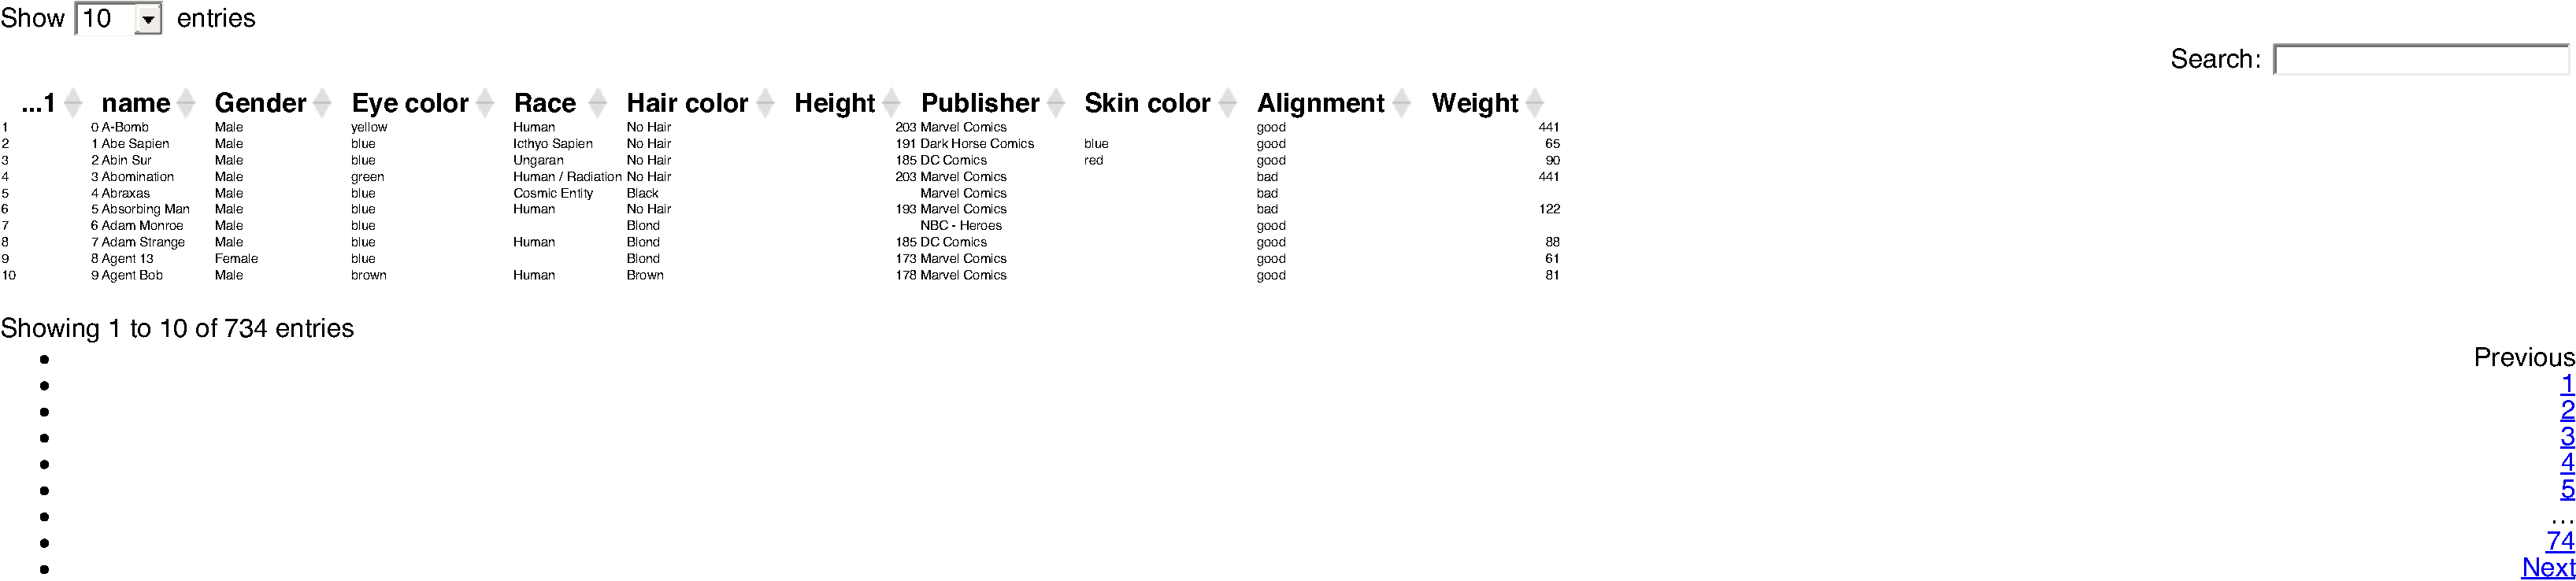
\includegraphics{smaller_autumn_quarto_files/figure-pdf/unnamed-chunk-6-1.pdf}

}

\end{figure}



\end{document}
